\documentclass[a4paper]{article}
\usepackage[T1]{fontenc}			% pacchetto per \chapter
\usepackage[italian]{babel}
\usepackage[italian]{isodate}  		% formato delle date in italiano
\usepackage{graphicx}				% gestione delle immagini
\usepackage{amsfonts}
\usepackage{booktabs}				% tabelle di qualità superiore
\usepackage{amsmath}				% pacchetto matematica
\usepackage{mathtools}				% per sottolineare sotto le equazioni
\usepackage{stmaryrd} 				% per '\llbracket' e '\rrbracket'
\usepackage{amsthm}					% teoremi migliorati
\usepackage{enumitem}				% gestione delle liste
\usepackage{pifont}					% pacchetto con elenchi carini
\usepackage{enumitem}				% pacchetto per elenchi con lettere dell'alfabeto
\usepackage{cancel}					% per cancellare delle espressioni matematiche
\usepackage{listings}				% implementa codice di programmazione


\usepackage[x11names]{xcolor}		% pacchetto colori RGB
% Link ipertestuali per l'indice
\usepackage{xcolor}
\usepackage[linkcolor=black, citecolor=blue, urlcolor=cyan]{hyperref}
\hypersetup{
	colorlinks=true
}

% Colour code style
\definecolor{codegreen}{rgb}{0,0.6,0}
\definecolor{codegray}{rgb}{0.5,0.5,0.5}
\definecolor{codepurple}{rgb}{0.58,0,0.82}
\definecolor{backcolour}{rgb}{0.95,0.95,0.92}

\lstdefinestyle{MATLAB}{
	backgroundcolor=\color{backcolour},   
	commentstyle=\color{codegreen},
	keywordstyle=\color{magenta},
	numberstyle=\tiny\color{codegray},
	stringstyle=\color{codepurple},
	basicstyle=\ttfamily\footnotesize,
	breakatwhitespace=false,         
	breaklines=true,                 
	captionpos=b,                    
	keepspaces=true,                 
	numbers=left,                    
	numbersep=5pt,
	showspaces=false,                
	showstringspaces=false,
	showtabs=false,                  
	tabsize=2
}
\lstset{style=MATLAB}

%\usepackage{showframe}				% visualizzazione bordi
%\usepackage{showkeys}				% visualizzazione etichetta

\newtheorem{theorem}{\textcolor{Red3}{\underline{Teorema}}}
\newtheorem{lemma}{Lemma}
\renewcommand{\qedsymbol}{QED}
\newcommand{\exec}[1]{\llbracket #1\:\rrbracket}
\newcommand{\dquotes}[1]{``#1''}
\newcommand{\longline}{\noindent\rule{\textwidth}{0.4pt}}

\begin{document}
	\author{Università degli Studi di Verona}
	\title{Simulazione di Elaborazione di segnali e immagini}
	\date{{\Large 14 Giugno 2021}}
	\maketitle
	
	\section{Esercizio (4 punti)}
	
	Data la seguente immagine:
	\begin{center}
		\begin{tabular}{| c | c | c | c | c | c | c |}
			\hline
			200 & 200 & 200 & 200 & 200 & 200 & 200 \\
			\hline
			200 & 200 & 200 & 200 & 200 & 200 & 200 \\
			\hline
			200 & 200 &  50 &  50 &  50 & 200 & 200 \\
			\hline
			200 & 200 &  50 &  50 &  50 & 200 & 200 \\
			\hline
			200 & 200 &  50 &  50 &  50 & 200 & 200 \\
			\hline
			200 & 200 & 200 & 200 & 200 & 200 & 200 \\
			\hline
			200 & 200 & 200 & 200 & 200 & 200 & 200 \\
			\hline
		\end{tabular}
	\end{center}
	Si applichi il seguente filtro:
	\begin{equation*}
		S = \dfrac{1}{4}\begin{bmatrix}
			 0 & -1 &  0 \\
			-1 &  8 & -1 \\
			 0 & -1 &  0
		\end{bmatrix}
	\end{equation*}
	Determina l'immagine filtrata \textbf{specificatamente in relazione ai suoi pixel in output di coordinate} $\left(2,2\right)$, $\left(3,3\right)$, $\left(4,4\right)$, effettuando un filtraggio "same" (ossia che preserva le dimensioni dell'immagine di input). Individua la natura del filtro (sharpening? Smoothing? Estrazione di edge?), motivando la scelta.
	
	\section{Esercizio (4 punti)}
	
	Definire analiticamente il seguente segnale e la sua trasformata di Fourier continua, determinando i seguenti valori del suo spettro di magnitudine, ovvero $f=0; f=0.5; f=1$ (la variabile $t$ indica il tempo, $f$ la frequenza).
	\begin{figure}[!htp]
		\centering
		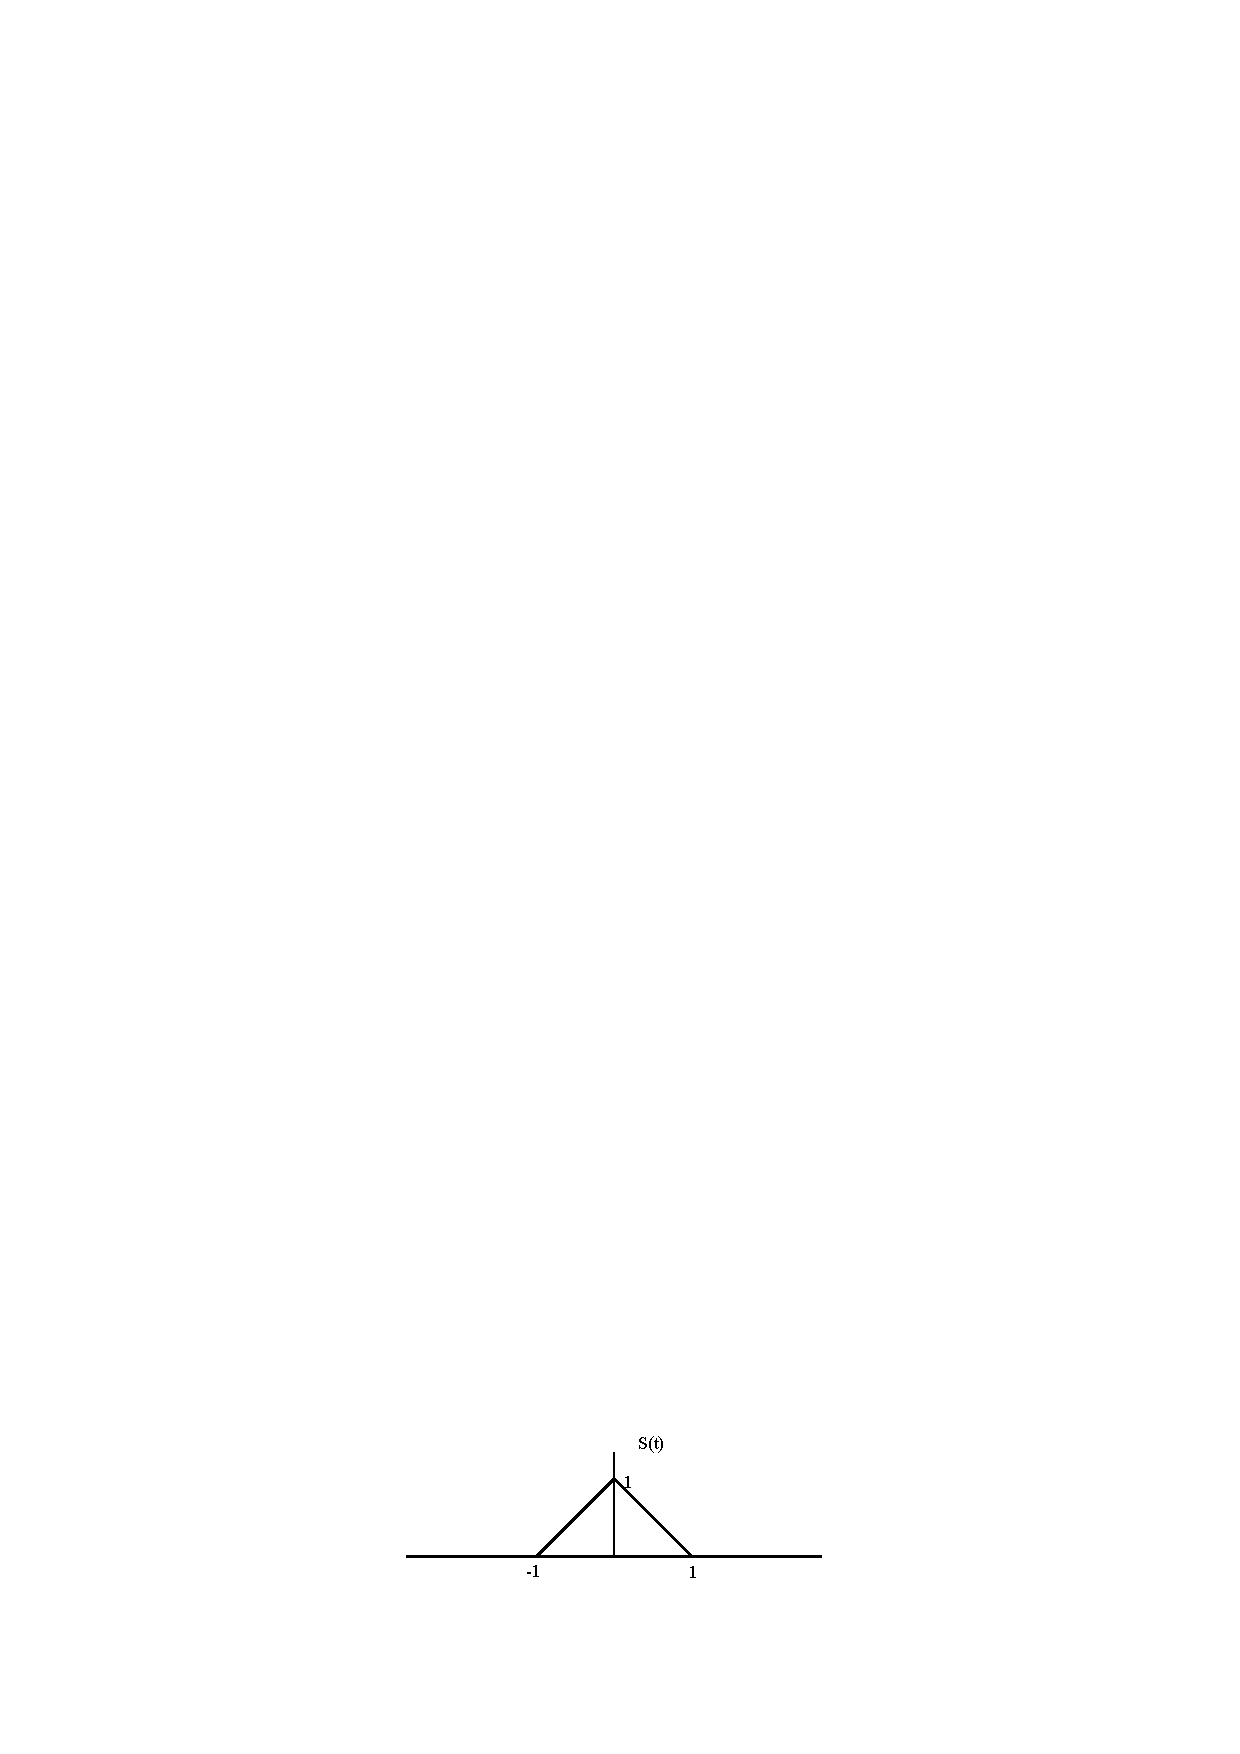
\includegraphics[width=.65\textwidth]{img/fig_1.pdf}
	\end{figure}\newpage

	\section{Esercizio (7 punti)}
	
	Si descriva analiticamente il segnale in frequenza mostrato nella figura sottostante, utilizzando le funzioni studiate a lezione.
	\begin{figure}[!htp]
		\centering
		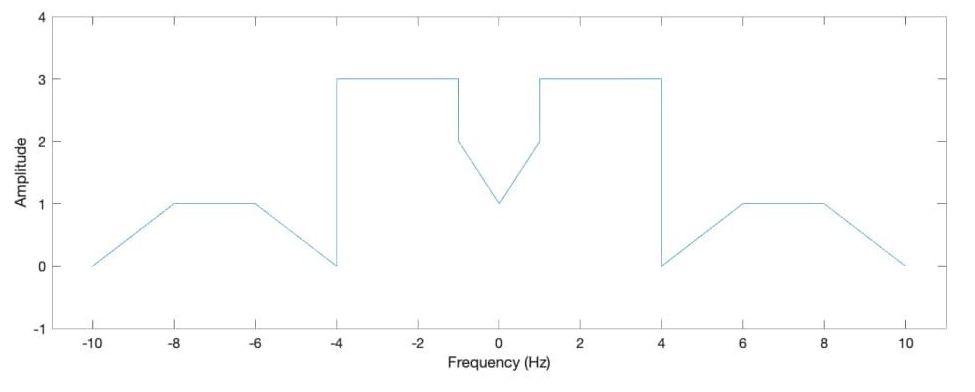
\includegraphics[width=\textwidth]{img/fig_2.png}
	\end{figure}

	\section{Esercizio (5 punti)}
	
	Si consideri il segnale:
	\begin{equation*}
		s\left(t\right) = \mathrm{sgn}\left(a \cdot \cos\left(\dfrac{2\pi}{T_{0}}t\right)\right)
	\end{equation*}
	E si risponda alle seguenti domande:
	\begin{enumerate}
		\item Rappresentare graficamente il segnale;
		\item Calcolare l'energia e la potenza del segnale e discutere se è un segnale a energia finita o a potenza finita.
	\end{enumerate}
	
	\section{Esercizio (5 punti)}
	
	Data la seguente immagine $3 \times 3$ mostrata di seguito, calcolare l'immagine dell'istogramma equalizzata (si supponga che i livelli di grigio siano nell'intervallo naturale $\left[0...7\right]$). Mostrare tutti i passaggi.
	\begin{center}
		\begin{tabular}{| c | c | c |}
			\hline
			3 & 1 & 1 \\
			\hline
			1 & 7 & 6 \\
			\hline
			0 & 2 & 1 \\
			\hline
		\end{tabular}
	\end{center}
\end{document}